\documentclass{beamer}
\usepackage[utf8]{inputenc}   % pour pouvoir taper les accents directement     
\usepackage{amsfonts,amssymb,amsmath}
\usepackage{tikz}
\usepackage{array}
\usepackage{calc}
\usetikzlibrary{patterns}
\usepackage[absolute,showboxes,overlay]{textpos}     
\textblockorigin{0pt}{0pt}                          
\TPshowboxesfalse  
 \usepackage{lmodern,multido}

\newcommand{\R}{\mathbb{R}}
\newcommand{\C}{\mathbb{C}}
\newcommand{\Z}{\mathbb{Z}}
\newcommand{\N}{\mathbb{N}}
\newcommand{\Q}{\mathbb{Q}}
\newcommand{\E}{(-4,-1) rectangle (4,4)}
\newcommand{\A}{(0,0) ++(135:2) circle (2)}
\newcommand{\B}{(0,0) ++(45:2) circle (2)}

\begin{document}
 %%%%%%%%%%%%%%%%%%%%%%%%%%%%%%%%%%%%%%%%%%%%%%%%%%%%%%%%%%%%%%%
  \addtobeamertemplate{navigation symbols}{}{ \hspace{1em}    \usebeamerfont{footline}%
    \insertframenumber/\inserttotalframenumber }
    
 %%%%%%%%%%%%%%%%%%%%%%%%%%%%%%%%%%%%%%%%%%%%%%%%%%%%%%%%%%%%%%%

\begin{frame}{Introduction aux statistiques}
\begin{textblock*}{\textwidth}(1cm,2cm)

\begin{center}{\bf \Large Chapitre 2} \end{center}
\begin{center}{\bf \Large Variables aléatoires continues} \end{center}
\vspace{0.3cm}
\begin{itemize}
\item Définition d'une variable aléatoire continue 
\item Caractéristiques d'une variable aléatoire continue
\item Lois usuelles discrètes 
\begin{itemize}
\item Loi uniforme
\item Loi exponentielle
\item Loi de Weibull
\item Loi Normale 
\end{itemize}
\end{itemize}

 \end{textblock*}

\end{frame}    
    
    
 %%%%%%%%%%%%%%%%%%%%%%%%%%%%%%%%%%%%%%%%%%%%%%%%%%%%%%%%%%%%%%%
\begin{frame}{Les variables aléatoires continues}

%{\Large Définition :}

La loi d'une v.a. continue est entièrement déterminée par sa {\bf densité de probabilité}  
$f : \mathbb{R}\longrightarrow \mathbb{R}$ telle que
$$
Pr(X\leq x)=\int_{-\infty}^x f(t) dt\,.
$$

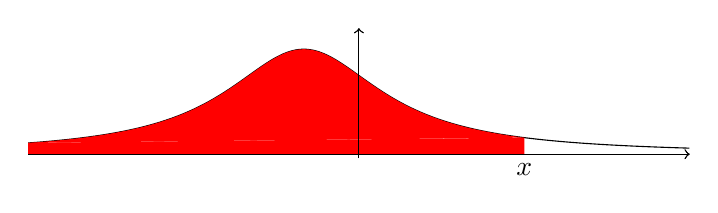
\begin{tikzpicture}[xscale=1.4,yscale=1]
\draw[->] (-3,0) -- (3,0);
\draw[->] (0,-0.05) -- (0,1.6);
%\draw (-2,-0.2) node {$a$};
\draw (1.5,-0.2) node {$x$};
\draw[domain=-3:3,samples=400] plot (\x,1/(1+\x*\x+\x) ;
\fill[color=red,domain=-3:1.5,samples=400] plot (\x,1/(1+\x*\x+\x) ;
\fill[color=red] (-3,0)--(-3,0.145)--(1.5,0.21)--(1.5,0);
\draw[->] (-3,0) -- (3,0);
\draw[->] (0,-0.05) -- (0,1.6);
\end{tikzpicture}

\

\begin{itemize}
\item $f$ est la dérivée de la fonction de répartition 
\item $\displaystyle \int_{-\infty}^{+\infty} f(t)dt =1$
\end{itemize}

 \end{frame}

 %%%%%%%%%%%%%%%%%%%%%%%%%%%%%%%%%%%%%%%%%%%%%%%%%%%%%%%%%%%%%%%
\begin{frame}{Les variables aléatoires continues}

%{\Large Définition :}

\begin{itemize}
\item  $\displaystyle  Pr(X\in [a\,;\,b])=\int_a^b f(t)dt$

\

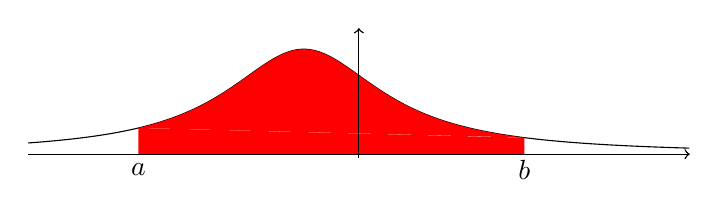
\begin{tikzpicture}[xscale=1.4,yscale=1]
\draw[->] (-3,0) -- (3,0);
\draw[->] (0,-0.05) -- (0,1.6);
\draw (-2,-0.2) node {$a$};
\draw (1.5,-0.2) node {$b$};
\draw[domain=-3:3,samples=400] plot (\x,1/(1+\x*\x+\x) ;
\fill[color=red,domain=-2:1.5,samples=400] plot (\x,1/(1+\x*\x+\x) ;
\fill[color=red] (-2,0)--(-2,0.3333)--(1.5,0.21)--(1.5,0);
\draw[->] (-3,0) -- (3,0);
\draw[->] (0,-0.05) -- (0,1.6);
\end{tikzpicture}
\end{itemize}


 \end{frame}

%%%%%%%%%%%%%%%%%%%%%%%%%%%%%%%%%%%%%%%%%%%%%

\begin{frame}{Les variables aléatoires continues}

%{\Large Variable continue :}

La loi d'une v.a. continue est entièrement déterminée par sa {\bf densité de probabilité} $f : \mathbb{R}\longrightarrow \mathbb{R}$ telle que
$$
Pr(X\leq x)=\int_{-\infty}^x f(t) dt\,.
$$
 
\ 




\end{frame}

%%%%%%%%%%%%%%%%%%%%%%%%%%%%%%%%%%%%%%%%%%%%%

\begin{frame}{Les variables aléatoires continues}

{\Large Caractéristiques d'une v.a. continue :}


\begin{itemize}
\item {\bf Espérance}  de $X$ :
$$
E(X)=\int_{-\infty}^{+\infty} tf(t) dt\,.
$$

\item {\bf Variance :} $Var(X)=E(X^2)-E(X)^2$ avec $$E(X^2)=\int_{-\infty}^{+\infty} t^2f(t) dt\,.$$

\item {\bf Écart-type :} $\sigma(X)=\sqrt{Var(X)}$.

\end{itemize}

\end{frame}

%%%%%%%%%%%%%%%%%%%%%%%%%%%%%%%%%%%%%%%%%%%%%

\begin{frame}{Les variables aléatoires continues}

\

\noindent {\bf \textcolor{red}{ Important :}} Avec une variable continue $X$ $$\forall \alpha\in \R, Pr(X=\alpha)=0.$$


On s'intéresse donc  plutôt aux probabilités $Pr(X\leq b)$, $Pr(X\geq a)$ ou $Pr(a\leq X\leq b)$. 

\

Remarque :  $P(X\leq b) =Pr(X<b)$.\\

\end{frame}

%%%%%%%%%%%%%%%%%%%%%%%%%%%%%%%%%%%%%%%%%%%%%

\begin{frame}{Les variables aléatoires continues}

\noindent {\bf Indépendance entre 2 v.a. continues :}

\

 $X$ et $Y$ continues sont indépendantes ssi pour tous intervalles $I$ et $J$ de $\R$ :
$$Pr(X\in I\;{\mbox { et }}\; Y\in J)=Pr(X\in I)\times Pr(Y\in J)\,.$$


\end{frame}


\begin{frame}{Lois usuelles continues}
\begin{textblock*}{\textwidth}(1cm,2cm)

\begin{center}{\bf \Large Loi Uniforme $U[a,b]$} \end{center}
\begin{itemize}
\item  densité de probabilité  :

\begin{minipage}{0.45\textwidth}
$$
f(x)=\left \{
\begin{array}{ll}
\frac{1}{b-a} & {\mbox {si } } x \in [a,b] \\
0 & {\mbox{sinon. }}
\end{array}
\right.
$$
\end{minipage}
\begin{minipage}{0.45\textwidth}
\begin{tikzpicture}[xscale=0.5,yscale=0.3]
\draw (2,-1) node {$a$};
\draw (5,-1) node {$b$};
\draw (-1,2) node {$\frac{1}{b-a}$};
\draw[->] (-0.5,0) -- (6,0);
\draw[->] (0,-0.5) -- (0,5.5);
\draw[-,color=red] (-0.5,0) -- (2,0);
\draw[-,color=red] (5,0) -- (6,0);
\draw[-,color=red] (2,2) -- (5,2);
\draw[-] (2,-0.4) -- (2,0.4);
\draw[-] (5,-0.4) -- (5,0.4);
\draw[-] (-0.2,2) -- (0.2,2);
\draw[dotted] (0.2,2) -- (2,2);
\draw[dotted] (2,0) -- (2,2);
\draw[dotted] (5,0) -- (5,2);
\end{tikzpicture}
\end{minipage}
\item fonction de répartition
\begin{center}
\begin{tikzpicture}[xscale=0.5,yscale=0.3]
\draw (2,-1) node {$a$};
\draw (5,-1) node {$b$};
\draw (-1,3) node {$1$};
\draw[->] (-0.5,0) -- (6,0);
\draw[->] (0,-0.5) -- (0,5.5);
\draw[-,color=red] (-0.5,0) -- (2,0);
\draw[-,color=red] (2,0) -- (5,3);
\draw[-,color=red] (5,3) -- (6,3);
\draw[-] (2,-0.4) -- (2,0.4);
\draw[-] (5,-0.4) -- (5,0.4);
\draw[-] (-0.2,3) -- (0.2,3);
\draw[dotted] (0.2,3) -- (5,3);
\draw[dotted] (5,0) -- (5,3);
\end{tikzpicture}
\end{center}
\end{itemize}

 \end{textblock*}

\end{frame}

 
 %%%%%%%%%%%%%%%%%%%%%%%%%%%%%%%%%%%%%%%%%%%%%%%%%%%%%%%%%%%%%%%

\begin{frame}{Lois usuelles continues}
\begin{textblock*}{\textwidth}(1cm,2cm)

\begin{center}{\bf \Large Loi Uniforme $U[a,b]$} \end{center}
\begin{itemize}
 \item $E(X)=\frac{a+b}{2}$ et $Var(X)=\frac{(a-b)^2}{12}$.\\
\end{itemize}

\

%\begin{minipage}{5.5cm}
%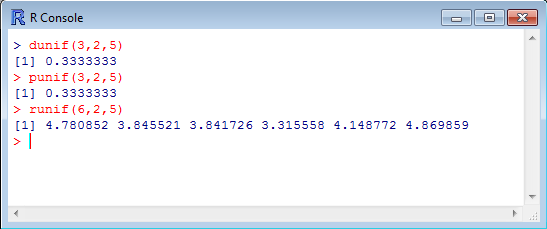
\includegraphics[width=5.5cm]{images/uniforme.png}
%\end{minipage}\ \ 
%\begin{minipage}{5cm}
%$X\sim U[2,5]$.
%\begin{itemize}
%\item calcul de $f(3)$ ;
%\item calcul de $P(X\leq 3)$ ;
%\item échantillon aléatoire de taille 6.
%\end{itemize}
%\end{minipage}


\end{textblock*}

\end{frame}

 %%%%%%%%%%%%%%%%%%%%%%%%%%%%%%%%%%%%%%%%%%%%%%%%%%%%%%%%%%%%%%%
\section{Loi exponentielle}

\begin{frame}{Lois usuelles continues}
\begin{textblock*}{\textwidth}(1cm,2cm)

\begin{center}{\bf \Large Loi exponentielle $\mathcal{E}(\lambda)$, avec $\lambda>0$} \end{center}
\begin{itemize}
\item  densité de probabilité  :
$
f(x)=
\begin{cases}
\lambda e^{-\lambda x}&\mbox { si }\quad  x\geq 0\, ;\\
0 & \mbox { si } \quad x<0.
\end{cases}
$

\item  fonction de répartition de $X$ :
$
F(x)=
\begin{cases}
1-e^{-\lambda x}&\mbox { si }\ x\geq 0\, ;\\
0 & \mbox { si } \  x<0.
\end{cases}
$
\begin{center}
\begin{tikzpicture}[xscale=0.9,yscale=0.4]
\draw[->] (-0.5,0) -- (2.5,0);
\draw[->] (0,-0.5) -- (0,4);
\draw[-] (-0.2,3) -- (0.2,3);
\draw (-0.5,3) node {$3$};
\draw[color=red] plot file {data/densite_exp.txt};
\end{tikzpicture}
\quad
\begin{tikzpicture}[xscale=0.9,yscale=0.3]
\draw (-0.5,3) node {$1$};
\draw[->] (-0.5,0) -- (2.5,0);
\draw[->] (0,-0.5) -- (0,5.5);
\draw[-] (-0.2,3) -- (0.2,3);
\draw[dotted] (0.2,3) -- (2.5,3);
\draw[color=red] plot file {data/repart_exp.txt};
\end{tikzpicture}
\end{center}

\end{itemize}

 \end{textblock*}

\end{frame}

 
 %%%%%%%%%%%%%%%%%%%%%%%%%%%%%%%%%%%%%%%%%%%%%%%%%%%%%%%%%%%%%%%

\begin{frame}{Lois usuelles continues}
\begin{textblock*}{\textwidth}(1cm,2cm)

\begin{center}{\bf \Large Loi exponentielle $\mathcal{E}(\lambda)$, avec $\lambda>0$} \end{center}
\begin{itemize}
 \item $E(X)=\sigma(X)=\frac{1}{\lambda}$
 
 \
 
 \item loi {\large \bf sans mémoire}
$$
Pr(X>t+\alpha \,|\, X>t)=P(X>\alpha)\,.
$$
\end{itemize}

\

%\begin{minipage}{5.5cm}
%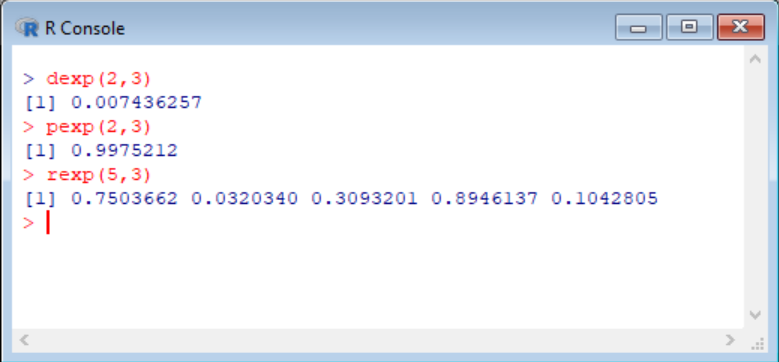
\includegraphics[width=5.5cm]{images/exponentiel.png}
%\end{minipage}\ \ 
%\begin{minipage}{5cm}
%$X\sim \mathcal{E}(3)$.
%\begin{itemize}
%\item calcul de $f(2)$ ;
%\item calcul de $P(X\leq 2)$ ;
%\item échantillon aléatoire de taille 5.
%\end{itemize}
%\end{minipage}


\end{textblock*}

\end{frame}

%%%%%%%%%%%%%%%%%%%%%%%%%%%%%%%%%%%%%%%%%%%%%%%%%%%%%%%%%%%%%%%

\section{Loi de Weibull}

\begin{frame}{Lois usuelles continues}
\begin{textblock*}{\textwidth}(1cm,2cm)

\begin{center}{\bf \Large Loi de Weibull $W(a,b)$ avec $a>0$ et $b>0$} \end{center}
\begin{itemize}
\item \small densité de probabilité  :
$
f(x)=
\begin{cases}
\frac{a}{b} \big( \frac{x}{b} \big)^{a-1} e^{ - \big( \frac{x}{b} \big)^{a} } &{\mbox { si }} x\geq 0\, ;\\
0 & \mbox { si } x<0.
\end{cases}
$
\end{itemize}


\begin{center}
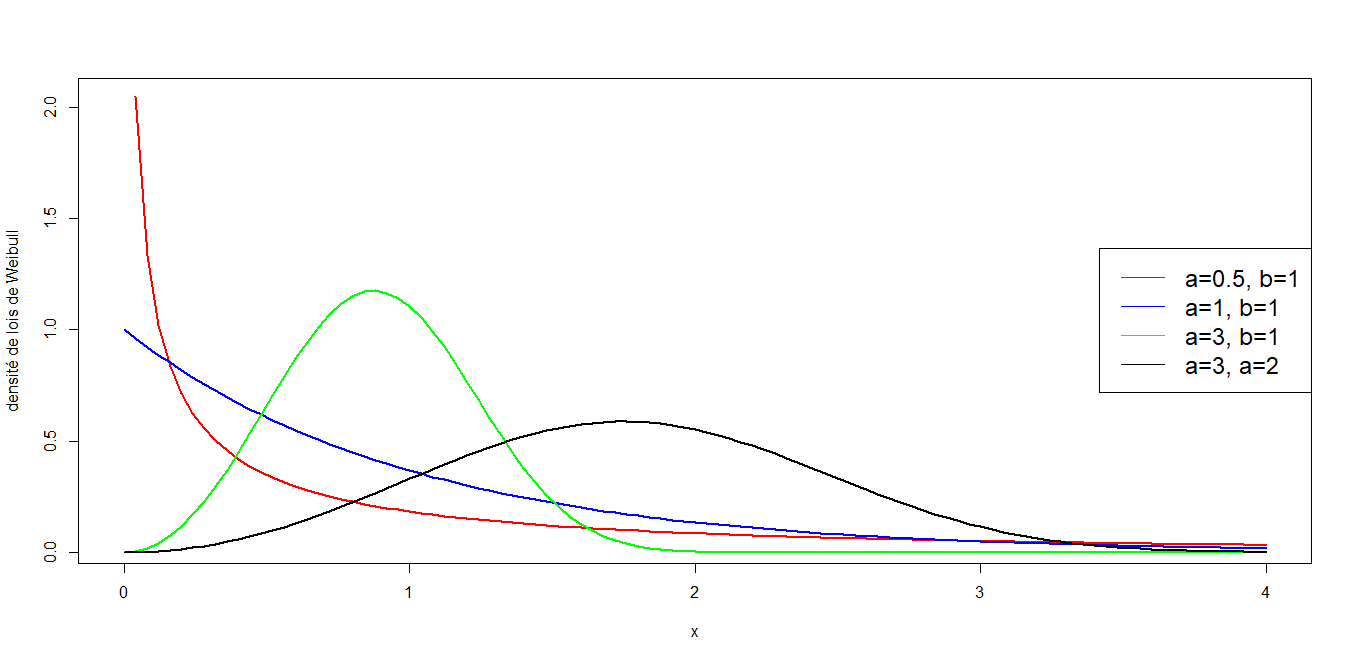
\includegraphics[scale=0.22]{images/densite_weibull.png}
\end{center}

\end{textblock*}

\end{frame}

%%%%%%%%%%%%%%%%%%%%%%%%%%%%%%%%%%%%%%%%%%%%%%%%%%%%%%%%%%%%%%%

\begin{frame}{Lois usuelles continues}
\begin{textblock*}{\textwidth}(1cm,2cm)

\begin{center}{\bf \Large Loi de Weibull $W(a,b)$ avec $a>0$ et $b>0$} \end{center}
\begin{itemize}

\item \small fonction de répartition de $X$ :
$
F(x)=
\begin{cases}
1- e^{ - \big( \frac{x}{b} \big)^{a} }& \mbox { si } \  x\geq 0;\\
0 & \mbox { si } \  x<0.
\end{cases}
$
\end{itemize}
\begin{center}
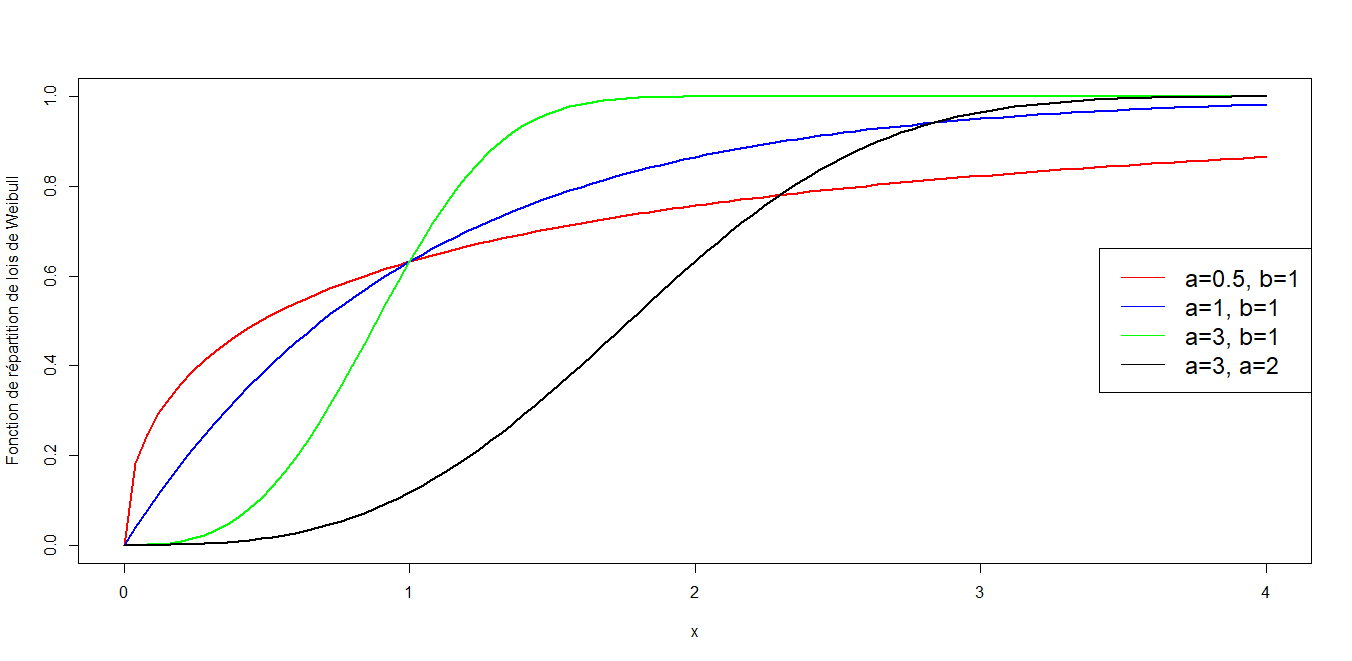
\includegraphics[scale=0.22]{images/Fdr_weibull.png}
\end{center}

\end{textblock*}

\end{frame} 

%%%%%%%%%%%%%%%%%%%%%%%%%%%%%%%%%%%%%%%%%%%%%%%%%%%%%%%%%%%%%%%

\begin{frame}{Lois usuelles continues}
\begin{textblock*}{\textwidth}(1cm,2cm)

\begin{center}{\bf \Large Loi de Weibull $W(a,b)$ avec $a>0$ et $b>0$} \end{center}


\begin{itemize}
\item 
 description de : 
 \begin{itemize}
\item durée de vie ;
\item temps d'attente avant panne ou accident.
\end{itemize}
\item  $a>1$ :  dégradation avec le temps ;
\item  $a<1$ :  bonification.

\end{itemize}


 
%\begin{minipage}{5.5cm}
%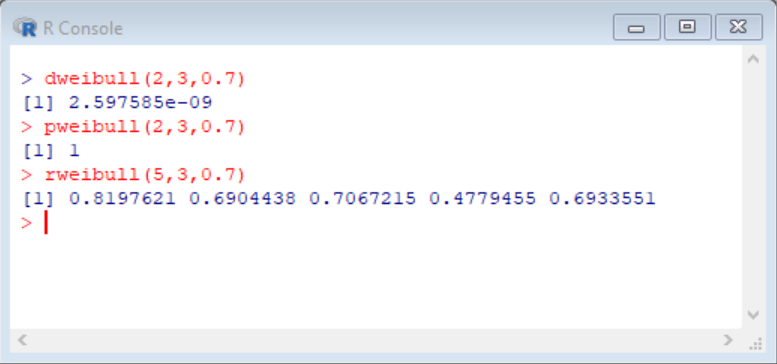
\includegraphics[width=5.5cm]{images/weibull.png}
%\end{minipage}\ \ 
%\begin{minipage}{5cm}
%$X\sim W(3,0.7)$.
%\begin{itemize}
%\item calcul de $f(2)$ ;
%\item calcul de $P(X\leq 2)$ ;
%\item échantillon aléatoire de taille 5.
%\end{itemize}
%\end{minipage}


\end{textblock*}

\end{frame}

%%%%%%%%%%%%%%%%%%%%%%%%%%%%%%%%%%%%%%%%%%%%%%%%%%%%%%%%%%%%%%%

\section{Loi normale}

\begin{frame}{Lois usuelles continues}
\begin{textblock*}{\textwidth}(1cm,2cm)

\begin{center}{\bf \Large Loi Normale $\mathcal{N}(\mu,\sigma)$ avec $\mu\in \mathbb{R}$ et $\sigma>0$} \end{center}
\begin{itemize}
\item ou loi gaussienne ou de Laplace-Gauss
\item approxime la somme de phénomènes aléatoires petits, nombreux et indépendants
\item essentielle en biologie  
\item loi limite des moyennes empiriques (théorème Central Limite)
\end{itemize}

 \end{textblock*}

\end{frame} 

%%%%%%%%%%%%%%%%%%%%%%%%%%%%%%%%%%%%%%%%%%%%%%%%%%%%%%%%%%%%%%%

\begin{frame}{Lois usuelles continues}
\begin{textblock*}{\textwidth}(1cm,1.5cm)

\begin{center}{\bf \Large Loi Normale $\mathcal{N}(\mu,\sigma)$ avec $\mu\in \mathbb{R}$ et $\sigma>0$} \end{center}
\begin{itemize}
\item \small densité de probabilité  :
$
f(x)=\frac{1}{\sigma\sqrt{2\pi}} e^{-\frac{(x-\mu)^2}{2\sigma^2}}
$

\begin{center}
\begin{minipage}{0.4\textwidth}
\begin{center}
\begin{tikzpicture}[xscale=0.7,yscale=0.8]
\draw[->] (-2.5,0) -- (2.5,0);
\draw[->] (0,-0.05) -- (0,2);
\draw[-] (-0.1,1) -- (0.1,1);
\draw (-0.5,1) node {$1$};
\draw[color=red] plot file {data/densite_norm_1.txt};
\end{tikzpicture}

$\mu=0$ et $\sigma=0.7$

\begin{tikzpicture}[xscale=0.7,yscale=0.8]
\draw[->] (-2.5,0) -- (2.5,0);
\draw[->] (0,-0.05) -- (0,2);
\draw[-] (-0.1,1) -- (0.1,1);
\draw (-0.5,1) node {$1$};
\draw[-] (1,-0.1) -- (1,0.1);
\draw (1,-0.5) node {$1$};
\draw[color=red] plot file {data/densite_norm_2.txt};
\end{tikzpicture}

$\mu=1$ et $\sigma=0.7$

\end{center}
\end{minipage}
\quad
\begin{minipage}{0.4\textwidth}
\begin{center}
\begin{tikzpicture}[xscale=0.7,yscale=0.8]
\draw[->] (-2.5,0) -- (2.5,0);
\draw[->] (0,-0.05) -- (0,2);
\draw[-] (-0.1,1) -- (0.1,1);
\draw (-0.5,1) node {$1$};
\draw[color=red] plot file {data/densite_norm_3.txt};
\end{tikzpicture}

$\mu=0$ et $\sigma=0.3$


\begin{tikzpicture}[xscale=0.7,yscale=0.8]
\draw[->] (-2.5,0) -- (2.5,0);
\draw[->] (0,-0.05) -- (0,2);
\draw[-] (-0.1,1) -- (0.1,1);
\draw (-0.5,1) node {$1$};
\draw[-] (1,-0.1) -- (1,0.1);
\draw (1,-0.5) node {$1$};
\draw[color=red] plot file {data/densite_norm_4.txt};
\end{tikzpicture}

$\mu=1$ et $\sigma=0.3$
\end{center}
\end{minipage}
\end{center}

\end{itemize}

 \end{textblock*}

\end{frame}


%%%%%%%%%%%%%%%%%%%%%%%%%%%%%%%%%%%%%%%%%%%%%%%%%%%%%%%%%%%%%%%

\begin{frame}{Lois usuelles continues}
\begin{textblock*}{\textwidth}(1cm,1.5cm)

\begin{center}{\bf \Large Loi Normale $\mathcal{N}(\mu,\sigma)$ avec $\mu\in \mathbb{R}$ et $\sigma>0$} \end{center}
\begin{itemize}
\item \small densité de probabilité  :
$
f(x)=\frac{1}{\sigma\sqrt{2\pi}} e^{-\frac{(x-\mu)^2}{2\sigma^2}}
$

\begin{center}
\begin{minipage}{0.3\textwidth}
\begin{center}
\begin{tikzpicture}[xscale=1,yscale=1]
\draw[->] (-0.05,0) -- (2.5,0);
\draw[->] (0,-0.05) -- (0,2);
\draw[-] (-0.1,1) -- (0.1,1);
\draw (-0.5,1) node {$1$};
\draw[color=red] plot file {data/densite_norm_5.txt};
\draw[dotted] (1,0.1) -- (1,1.25) ;
\draw (1,0.1) -- (1,-0.1) ;
\draw (1,-0.5) node {$1$};
\end{tikzpicture}

$\mu=1$ et $\sigma=0.3$

\end{center}
\end{minipage}
\quad
\begin{minipage}{0.55\textwidth}
\begin{itemize}
\item courbe {\it en cloche}
\item symétrique autour de la moyenne $\mu$
\item  beaucoup de sujets autour de la valeur moyenne
\item nombre décroissant quand on s'éloigne
de $\mu$.
\item décroit d'autant plus vite que $\sigma$ petit
\end{itemize}
\end{minipage}
\end{center}

\end{itemize}

 \end{textblock*}

\end{frame}

%%%%%%%%%%%%%%%%%%%%%%%%%%%%%%%%%%%%%%%%%%%%%%%%%%%%%%%%%%%%%%%

\begin{frame}{Lois usuelles continues}
\begin{textblock*}{\textwidth}(1cm,2cm)

\begin{center}{\bf \Large Loi Normale $\mathcal{N}(\mu,\sigma)$ avec $\mu\in \mathbb{R}$ et $\sigma>0$} \end{center}

\begin{itemize}
\item \small fonction de répartition de $X$ :
\end{itemize}

\begin{center}
\begin{tikzpicture}[xscale=0.5,yscale=0.45]
\draw (-0.5,3) node {$1$};
\draw[->] (-1,0) -- (5,0);
\draw[->] (0,-0.5) -- (0,4.5);
\draw[-] (-0.2,3) -- (0.2,3);
\draw[dotted] (0.2,3) -- (2.5,3);
\draw[dotted] (1,0.1) -- (1,1.5) ;
\draw[dotted] (0.1,1.5) -- (1,1.5) ;
\draw (1,0.1) -- (1,-0.1) ;
\draw (1,-0.5) node {$1$};
\draw (0.1,1.5) -- (-0.1,1.5) ;
\draw (-0.8,1.5) node {$0.5$};
\draw[color=red] plot file {data/repart_norm.txt};
\end{tikzpicture}

$\mu=1$ et $\sigma=0.3$
\end{center}

 \end{textblock*}

\end{frame} 

%%%%%%%%%%%%%%%%%%%%%%%%%%%%%%%%%%%%%%%%%%%%%%%%%%%%%%%%%%%%%%%


\begin{frame}{Lois usuelles continues}
\begin{textblock*}{\textwidth}(1cm,2cm)

\begin{center}{\bf \Large Loi Normale $\mathcal{N}(\mu,\sigma)$ avec $\mu\in \mathbb{R}$ et $\sigma>0$} \end{center}

\

\begin{itemize}
\item  $E(X)=\mu$ et $Var(X)=\sigma^2$

\

\item loi normale :  mode (valeur où maximum de densité de probabilité) = moyenne = médiane =$\mu$
\end{itemize}


 
%\begin{minipage}{5.5cm}
%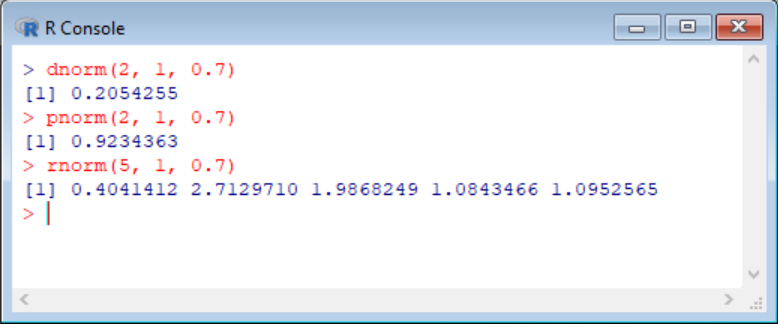
\includegraphics[width=5.5cm]{images/norm.png}
%\end{minipage}\ \ 
%\begin{minipage}{5cm}
%$X\sim \mathcal{N}(1,0.7)$.
%\begin{itemize}
%\item calcul de $f(2)$ ;
%\item calcul de $P(X\leq 2)$ ;
%\item échantillon aléatoire de taille 5.
%\end{itemize}
%\end{minipage}


\end{textblock*}

\end{frame}

%%%%%%%%%%%%%%%%%%%%%%%%%%%%%%%%%%%%%%%%%%%%%%%%%%%%%%%%%%%%%%%


\begin{frame}{Lois usuelles continues}
\begin{textblock*}{\textwidth}(1cm,1cm)

\begin{center}{\bf \Large Loi Normale centrée réduite $\mathcal{N}(0,1)$} \end{center}

\begin{itemize}
%\item $\mathcal{N}(0,1)$ loi normale {\large \bf  centrée réduite}
\item Des tables numériques donnent $Pr(X<a)$ ou $Pr(|X|>a)$ pour $X\sim \mathcal{N}(0,1)$

\item Symétrie par rapport à 0 :

\vspace{-1mm}$$Pr(X<-a)=Pr(X>a)=1-Pr(X<a)$$

\item Toute loi $\mathcal{N}(\mu,\sigma)$ peut être ramenée à une loi $\mathcal{N}(0,1)$ : \\
si $X\sim\mathcal{N}(\mu,\sigma)$ alors  $Z=\displaystyle \frac{X-\mu }{\sigma}\sim \mathcal{N}(0,1)$

\item Pour calculer des probabilités associées à $X$ :
$$
Pr(X<a) = Pr\left( \frac{X-\mu}{\sigma} < \frac{a-\mu}{\sigma}\right) = Pr\left(Z< \frac{a-\mu}{\sigma} \right)
$$

\end{itemize}

\end{textblock*}

\end{frame}



%%%%%%%%%%%%%%%%%%%%%%%%%%%%%%%%%%%%%%%%%%%%%%%%%%%%%%%%%%%%%%%
%%%%%%%%%%%%%%%%%%%%%%%%%%%%%%%%%%%%%%%%%%%%%%%%%%%%%%%%%%%%%%%


\begin{frame}{Lois usuelles continues}
\begin{textblock*}{\textwidth}(1cm,1.5cm)

%\begin{center}{\bf \Large Loi Normale $\mathcal{N}(\mu,\sigma)$ avec $\mu\in \mathbb{R}$ et $\sigma>0$} %\end{center}

Table de la fonction de répartition de la loi Normale centrée réduite \\ donnant $P(X<x)$ pour $X\sim \mathcal{N}(0,1)$ : \\

\

\includegraphics[scale=0.43]{images/table_norm_CR.png}

\end{textblock*}

\end{frame}

%%%%%%%%%%%%%%%%%%%%%%%%%%%%%%%%%%%%%%%%%%%%%%%%%%%%%%%%%%%%%%%




\begin{frame}{Lois usuelles continues}
\begin{textblock*}{\textwidth}(1cm,1cm)

\begin{center}{\bf \Large Somme de v.a. Normales} \end{center}

\begin{itemize}
\item Si $X_1\sim \mathcal{N}(\mu_1,\sigma_1)$ et $X_2\sim\mathcal{N}(\mu_2,\sigma_2)$, indépendantes, alors
 $$X_1 + X_2\sim \mathcal{N}\left(\mu_1+\mu_2,\sqrt{\sigma_1^2+\sigma_2^2}\right)$$

\item Avec $\alpha, \beta \in \R$, alors
 $$\alpha X_1 + \beta X_2\sim \mathcal{N}\left(\alpha\mu_1+\beta\mu_2,\sqrt{\alpha^2\sigma_1^2+\beta^2\sigma_2^2}\right)$$

\item Si n v.a. Normales $X_i\sim \mathcal{N}(\mu_i,\sigma_i)$, pour $i=\{1, ...n\}$, alors :
 $$\sum_{i=1}^n X_i \sim \mathcal{N}\left(\sum_{i=1}^n \mu_i,\sqrt{\sum_{i=1}^n \sigma_i^2}\right)$$
\end{itemize}


\end{textblock*}

\end{frame}

%%%%%%%%%%%%%%%%%%%%%%%%%%%%%%%%%%%%%%%%%%%%%%%%%%%%%%%%%%%%%%%


\begin{frame}{Lois usuelles continues}
\begin{textblock*}{\textwidth}(1cm,2cm)

\begin{center}{\bf \Large Loi Normale $\mathcal{N}(\mu,\sigma)$ avec $\mu\in \mathbb{R}$ et $\sigma>0$} \end{center}



\begin{itemize}
\item {\bf Intervalles importants :} si $X\sim\mathcal{N}(\mu,\sigma)$ :
\only<1>
{$Pr(\mu-1,96\times \sigma \leq X \leq \mu+1,96\times \sigma)  \approx  0,95$}
\only<2>
{$Pr(\mu-2,576 \times\sigma \leq X \leq \mu+2,576 \times \sigma)  \approx  0,99$}
\only<3>
{$Pr(\mu-3,29 \times \sigma \leq X \leq \mu+3,29 \times\sigma)  \approx  0,999$}



\begin{center}
\begin{tikzpicture}[xscale=2,yscale=2]
\draw[->] (-0.1,0) -- (3,0);
\draw[->] (0,-0.05) -- (0,1.4);
\only<1>
{
\draw (0.5,-0.2) node {$\mu-1,96\sigma$};
\draw (1.8,-0.2) node {$\mu+1,96\sigma$};
\draw[red] (2,1) node {$95\%$};
\draw plot file {data/densite_norm_95.txt} -- cycle;
\fill[color=red] plot file {data/densite_norm_95.txt} -- cycle;
}
\only<2>
{
\draw (0.3,-0.2) node {$\mu-2,576\sigma$};
\draw (2,-0.2) node {$\mu+2,576\sigma$};
\draw[red] (2,1) node {$99\%$};
\draw plot file {data/densite_norm_99.txt} -- cycle;
\fill[color=red] plot file {data/densite_norm_99.txt} -- cycle;
}
\only<3>
{
\draw (0,-0.2) node {$\mu-3,29\sigma$};
\draw (2.2,-0.2) node {$\mu+3,29\sigma$};
\draw[red] (2,1) node {$99,9\%$};
\draw plot file {data/densite_norm_999.txt} -- cycle;
\fill[color=red] plot file {data/densite_norm_999.txt} -- cycle;
}

\draw plot file {data/densite_norm_5.txt};
\end{tikzpicture}

\end{center}

\end{itemize}

\end{textblock*}

\end{frame}


%%%%%%%%%%%%%%%%%%%%%%%%%%%%%%%%%%%%%%%%%%%%%%%%%%%%%%%%%%%%%%%


\begin{frame}{Lois usuelles continues}
\begin{textblock*}{\textwidth}(1cm,2cm)

\begin{center}{\bf \Large Loi Normale $\mathcal{N}(\mu,\sigma)$ avec $\mu\in \mathbb{R}$ et $\sigma>0$} \end{center}

Table des valeurs extrêmes la loi Normale centrée réduite donnant $P(|X|>z_{\alpha})=\alpha$ pour $X\sim \mathcal{N}(0,1)$ : \\

\includegraphics[scale=0.7]{images/table_norm_CR2.png}

\end{textblock*}

\end{frame}

\end{document}
 %%%%%%%%%%%%%%%%%%%%%%%%%%%%%%%%%%%%%%%%%%%%%%%%%%%%%%%%%%%%%%%

\begin{frame}{Lois usuelles continues}
\begin{textblock*}{\textwidth}(1cm,2cm)

\begin{center}{\bf \Large Loi Log-Normale $Log-\mathcal{N}(\mu,\sigma)$ avec $\mu\in \mathbb{R}$ et $\sigma>0$} \end{center}
\begin{itemize}
\item $X\sim Log-\mathcal{N}(\mu,\sigma)$ ssi $\ln(X)\sim \mathcal{N}(\mu,\sigma)$
\item  densité de probabilité  :
$
f(x)=
\begin{cases}
\frac{1}{\sigma x\sqrt{2\pi}} e^{-\frac{(\ln (x) -\mu)^2}{2\sigma^2}}&\mbox { si }\quad  x> 0\, ;\\
0 & \mbox { si } \quad x\leq 0.
\end{cases}
$
\end{itemize}

\begin{center}
\begin{tikzpicture}[xscale=0.4,yscale=2]
\draw[->] (-0.5,0) -- (9,0);
\draw[->] (0,-0.1) -- (0,0.7);
\draw[color=red] plot file {data/densite_lognorm.txt};
\end{tikzpicture}

\end{center}



 \end{textblock*}

\end{frame}

 
 %%%%%%%%%%%%%%%%%%%%%%%%%%%%%%%%%%%%%%%%%%%%%%%%%%%%%%%%%%%%%%%

\begin{frame}{Lois usuelles continues}
\begin{textblock*}{\textwidth}(1cm,2cm)


\begin{center}{\bf \Large Loi Log-Normale $Log-\mathcal{N}(\mu,\sigma)$ avec $\mu\in \mathbb{R}$ et $\sigma>0$} \end{center}

Si $X\sim Log-\mathcal{N}(\mu,\sigma) $
\begin{itemize}
 \item  $E(X)=e^{(\mu+\sigma^2/2)}$ ; $\sigma^2(X)=(e^{\sigma^2}-1) e^{2\mu+\sigma^2}$
 \item mode $e^{(\mu-\sigma^2)}$.

\end{itemize}

\

\begin{minipage}{5.5cm}
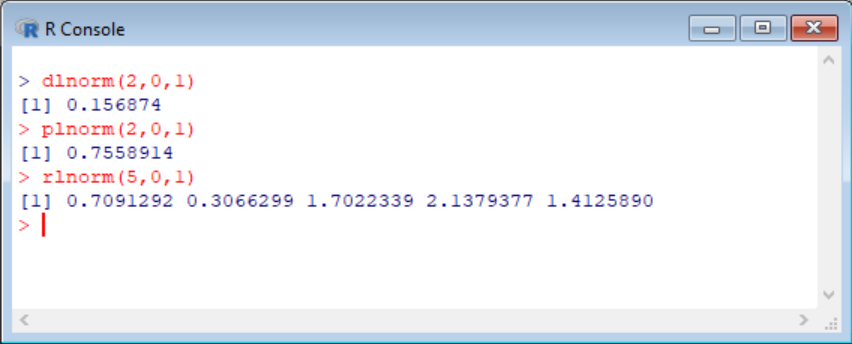
\includegraphics[width=5.5cm]{images/lognorm.png}
\end{minipage}\ \ 
\begin{minipage}{5cm}
$X\sim Log-\mathcal{N}(0,1)$.
\begin{itemize}
\item calcul de $f(2)$ ;
\item calcul de $P(X\leq 2)$ ;
\item échantillon aléatoire de taille 5.
\end{itemize}
\end{minipage}


\end{textblock*}

\end{frame}

 %%%%%%%%%%%%%%%%%%%%%%%%%%%%%%%%%%%%%%%%%%%%%%%%%%%%%%%%%%%%%%%

\begin{frame}{Lois usuelles continues}
\begin{textblock*}{\textwidth}(1cm,2cm)

\begin{center}{\bf \Large Loi Log-Normale $Log-\mathcal{N}(\mu,\sigma)$ avec $\mu\in \mathbb{R}$ et $\sigma>0$} \end{center}


Utilisée pour modéliser 
\begin{itemize}
\item la distribution du poids ;
\item le dosage de certains médicaments
\item le temps de survie de bactéries...
\item des observations résultant d'un effet multiplicatif 
d'un  grand nombre de variables indépendantes  et individuellement négligeables.
\end{itemize}




\end{textblock*}

\end{frame}

%%%%%%%%%%%%%%%%%%%%%%%%%%%%%%%%%%%%%%%%%%%%%%%%%%%%%%%%%%%%%%%

\begin{frame}{Lois usuelles continues}
\begin{textblock*}{\textwidth}(1cm,2cm)

\begin{center}{\bf \Large Loi du $\chi^2$} \end{center}
\begin{itemize}
\item \small densité de probabilité :
$
f(x)=
\begin{cases}
\frac{1}{2^\frac{d}{2} \Gamma\left(\frac{d}{2}\right)} x^{\frac{d}{2}-1} e^{-x/2} &{\mbox { si }} x> 0\, ;\\
0 & \mbox { si } x\leq0.
\end{cases}
$

\begin{center}
\begin{minipage}{0.4\textwidth}
\begin{center}
\begin{tikzpicture}[xscale=0.7,yscale=0.7]
\draw[->] (-0.5,0) -- (5,0);
\draw[->] (0,-0.05) -- (0,2.1);
\draw[-] (-0.1,1) -- (0.1,1);
\draw (-0.5,1) node {$1$};
\draw[color=red] plot file {data/densite_chi_1.txt};
\end{tikzpicture}

$1ddl$

\begin{tikzpicture}[xscale=0.7,yscale=2.2]
\draw[->] (-0.5,0) -- (5,0);
\draw[->] (0,-0.05) -- (0,0.6);
\draw[-] (-0.1,0.5) -- (0.1,0.5);
\draw (-0.5,0.5) node {$0.5$};
\draw[color=red] plot file {data/densite_chi_3.txt};
\end{tikzpicture}

$3ddl$
\end{center}
\end{minipage}
\quad
\begin{minipage}{0.4\textwidth}
\begin{center}
\begin{tikzpicture}[xscale=0.7,yscale=2.6]
\draw[->] (-0.5,0) -- (5,0);
\draw[->] (0,-0.05) -- (0,0.6);
\draw[-] (-0.1,0.5) -- (0.1,0.5);
\draw (-0.5,0.5) node {$0.5$};
\draw[color=red] plot file {data/densite_chi_2.txt};
\end{tikzpicture}

$2ddl$

\begin{tikzpicture}[xscale=0.7,yscale=2.2]
\draw[->] (-0.5,0) -- (5,0);
\draw[->] (0,-0.05) -- (0,0.6);
\draw[-] (-0.1,0.5) -- (0.1,0.5);
\draw (-0.5,0.5) node {$0.5$};
\draw[color=red] plot file {data/densite_chi_4.txt};
\end{tikzpicture}

$4ddl$
\end{center}
\end{minipage}
\end{center}

\end{itemize}

 \end{textblock*}

\end{frame}

%%%%%%%%%%%%%%%%%%%%%%%%%%%%%%%%%%%%%%%%%%%%%%%%%%%%%%%%%%%%%%%

\begin{frame}{Lois usuelles continues}
\begin{textblock*}{\textwidth}(1cm,2cm)

\begin{center}{\bf \Large Loi du $\chi^2$} \end{center}
\begin{itemize}
\item $Y$ suit une loi du $\chi^2$ à $d$ degrés de liberté si 
\begin{center}$
Y=X_1^2 + X_2^2 + \hdots + X_d^2
$\end{center}
où les $X_i$ sont indépendantes et $X_i \sim \mathcal{N}(0;1)$.

\item $E(Y)=d$ et $Var(Y)=2d$.\\
\end{itemize}


\begin{minipage}{5.5cm}
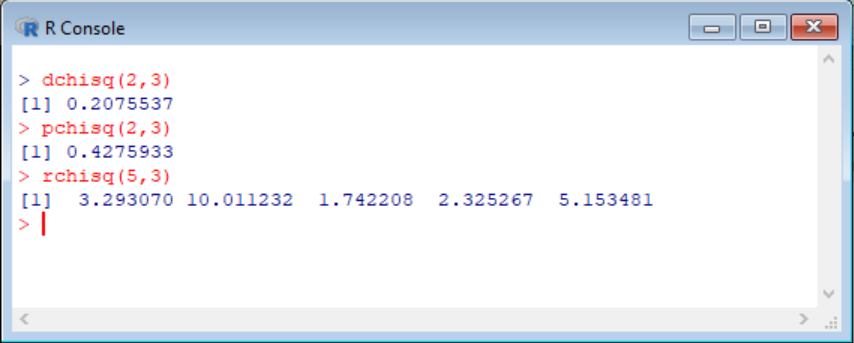
\includegraphics[width=5.5cm]{images/chi.png}
\end{minipage}\ \ 
\begin{minipage}{5cm}
$X$ suit  loi du $\chi^2$ à 3 ddl.
\begin{itemize}
\item calcul de $f(2)$ ;
\item calcul de $P(X\leq 2)$ ;
\item échantillon aléatoire de taille 5.
\end{itemize}
\end{minipage}
 \end{textblock*}

\end{frame}


%%%%%%%%%%%%%%%%%%%%%%%%%%%%%%%%%%%%%%%%%%%%%%%%%%%%%%%%%%%%%%%

\begin{frame}{Lois usuelles continues}
\begin{textblock*}{\textwidth}(1cm,2cm)

\begin{center}{\bf \Large Loi de Student} \end{center}
\begin{itemize}
\item \small densité de probabilité :
$
f(x)=
\frac{1}{\sqrt{\pi d}} \frac{\Gamma(\frac{d+1}{2})}{\Gamma(\frac{d}{2})} 
\frac{1}{(1+\frac{x^2}{d})^{\frac{d+1}{2}}}
$
\end{itemize}

\begin{center}
\begin{minipage}{0.4\textwidth}
\begin{center}
\begin{tikzpicture}[xscale=0.7,yscale=2]
\draw[->] (-2.5,0) -- (2.5,0);
\draw[->] (0,-0.05) -- (0,0.6);
\draw[-] (-0.1,0.5) -- (0.1,0.5);
\draw (-0.5,0.5) node {$0.5$};
\draw[color=red] plot file {data/densite_student_3.txt};
\draw[color=green,dashed] plot file {data/densite_norm_01.txt};
\end{tikzpicture}

$3 ddl$
\end{center}
\end{minipage}
\quad
\begin{minipage}{0.4\textwidth}
\begin{center}
\begin{tikzpicture}[xscale=0.7,yscale=2]
\draw[->] (-2.5,0) -- (2.5,0);
\draw[->] (0,-0.05) -- (0,0.6);
\draw[-] (-0.1,0.5) -- (0.1,0.5);
\draw (-0.5,0.5) node {$0.5$};
\draw[color=red] plot file {data/densite_student_30.txt};
\draw[color=green,dashed] plot file {data/densite_norm_01.txt};
\end{tikzpicture}

$df=30ddl$
\end{center}
\end{minipage}
\end{center}

\begin{itemize}
\item si $T$ suit une loi de Student à $d$ degrés de liberté avec $d$ grand ($d>30$ par exemple) 
alors $T$ suit approximativement une loi normale centrée réduite $\mathcal{N}(0;1)$.
\end{itemize}

 \end{textblock*}

\end{frame}


\end{document}

%%%%%%%%%%%%%%%%%%%%%%%%%%%%%%%%%%%%%%%%%%%%%%%%%%%%%%%%%%%%%%%

\begin{frame}{Lois usuelles continues}
\begin{textblock*}{\textwidth}(1cm,2cm)

\begin{center}{\bf \Large Loi de Student} \end{center}
\begin{itemize}
\item  $T$ suit une loi de Student à $d$ degrés de liberté si $T=\frac{X}{\sqrt{Y/d}}$ 

\begin{itemize}
\item  $X\sim \mathcal{N}(0;1)$ ; 
\item  $Y$ suit une loi du $\chi^2$ à 
$d$ degrés de liberté ;
\item  $X$ et $Y$  indépendantes.
\end{itemize}

\item $E(T)=0$ si $d>1$ ; $Var(T)=\frac{d}{d-2}$ si $d>2$.
\end{itemize}


\begin{minipage}{5.5cm}
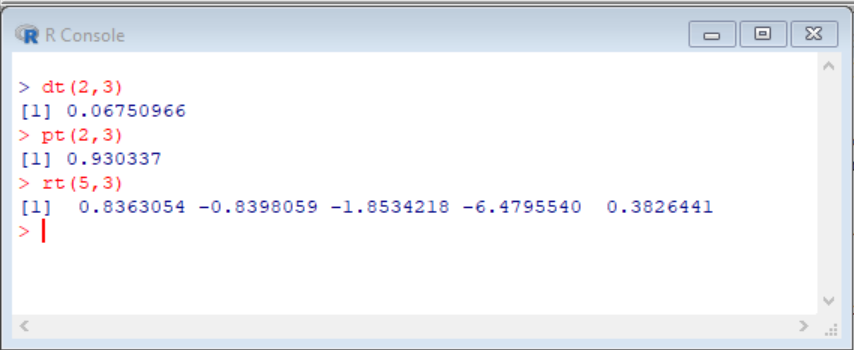
\includegraphics[width=5.5cm]{images/student.png}
\end{minipage}\ \ 
\begin{minipage}{5cm}
$X$ suit loi de Student à 3 ddl.
\begin{itemize}
\item calcul de $f(2)$ ;
\item calcul de $P(X\leq 2)$ ;
\item échantillon aléatoire de taille 5.
\end{itemize}
\end{minipage}
 \end{textblock*}

\end{frame}


\end{document}













 








